%******************************************************************************%
%                                                                              %
%                                 Interlude                                    %
%                         for Machine Learning module                          %
%                                                                              %
%******************************************************************************%

% =============================== %
\section*{Interlude}
% =============================== %
\subsection*{Predict II : Hypothesis}
% ------------------------------- %

We hope your curiosity led you to plot your sigmoid function.
If you didn't, well here is what it looks like:

\begin{figure}[!h]
    \centering
    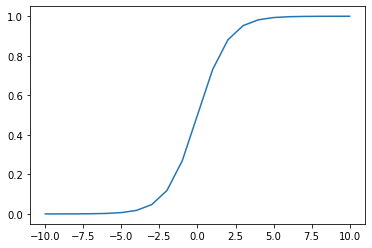
\includegraphics[scale=0.55]{assets/sigmoid.png}
    \caption{Sigmoid}
\end{figure}
As you can see, \textbf{the sigmoid's output values range from $0$ to $1$}.\\
\\
You can input real numbers as big as you want (positive or negative), the output 
will always land within this range.
This will be very helpful and convenient for the next part.

\newpage

% =============================== %
\subsection*{Logistic Hypothesis}
% ------------------------------- %

Now you've written your sigmoid function, let's take a look at \textbf{the logistic regression
 hypothesis}.

$$
\begin{matrix}
\hat{y}^{(i)} & = & h_\theta(x^{(i)}) & = & \text{sigmoid}(\theta \cdot x'^{(i)}) 
& =  &\cfrac{1} {1 + e^{-\theta \cdot x'^{(i)}}} & &\text{ for i = 1, \dots, m}    
\end{matrix}
$$
\textbf{This is simply the sigmoid function applied on top 
of the linear regression hypothesis!!}\\
\\
It can be vectorized as:
\\
$$
\begin{matrix}
\hat{y} & = & h_\theta(X) & = & \text{sigmoid}(X'\theta) & =  &\cfrac{1} {1 + e^{-X'\theta}}    
\end{matrix}
$$
As we said before: the \textbf{sigmoid function} is just a way 
to \textbf{map the result of a linear equation onto a $[0,1]$ value range}.\\
\\
This transformation allows us to interpret the result 
as a \textbf{probability that an individual or observation belongs to of a given class}.\\